\section{Problem Formulation}\label{sec:problem}

\subsection{Spatial Cells, Candidate Viewpoints, and Feasible Coverage}

Let $\mathcal R=\{1,\ldots,N\}$ be the set of directional camera devices. The evaluation region is represented by $M$ equal-weight cell centers $\mathcal C=\{\mathbf x_m\}_{m=1}^{M}$. Device $i$ has a finite candidate-viewpoint set $\mathcal Q_i$. A viewpoint $q=(\theta_{iq},\phi_{iq})$ specifies azimuth and elevation in the device's control coordinate system. Given the device pose, mounting rotation, camera intrinsics, and fixed zoom, the pinhole model maps each candidate to a nominal cell set $\mathcal B_{iq}$. These quantities define a common frozen geometry for all compared planning methods.

The planner operates on an admissible map $\mathcal B^{\mathrm a}_{iq}\subseteq\mathcal B_{iq}$. This separation is useful because the propositions require only that all methods use the same frozen map; they do not require a particular construction. In the hardware implementation, the map was generated from the completion tolerance of the pose controller. Let
$\mathcal D_i=[-e_i^\theta,e_i^\theta]\times[-e_i^\phi,e_i^\phi]$, where $e_i^\theta$ and $e_i^\phi$ are azimuth and elevation half-widths and $\operatorname{corners}(\mathcal D_i)$ denotes the four corners of the error box. The implemented planning core is

\begin{equation}\label{eq:safety-core}
\mathcal B^{\mathrm s}_{iq}=
\bigcap_{(\delta_\theta,\delta_\phi)\in\operatorname{corners}(\mathcal D_i)}
\mathcal B_i(\theta_{iq}+\delta_\theta,\phi_{iq}+\delta_\phi),
\qquad \mathcal B^{\mathrm a}_{iq}=\mathcal B^{\mathrm s}_{iq}.
\end{equation}

Equation~\eqref{eq:safety-core} is a practical four-corner intersection used by the frozen implementation. It reduces dependence on cells lying at the nominal field-of-view boundary. It is not a physical confidence region for the camera footprint: station coordinates, mounting extrinsics, and per-camera intrinsic errors were not jointly calibrated against external ground truth. It is also not the principal algorithmic contribution. Replacing it with another frozen feasible map would leave the baseline-preserving proofs unchanged, provided that all compared plans were evaluated on that same map.

A route for device $i$ is an ordered sequence $\pi_i=(q_{i1},\ldots,q_{iK_i})$, and a team plan is $\Pi=\{\pi_i\}_{i=1}^{N}$. The planning task is feasible only if the union of admissible candidate sets covers all cells. Feasibility is checked before route construction. During execution, $\mathcal B^{\mathrm a}_{iq}$ can justify assigning a viewpoint but cannot itself create a realized coverage record; that record is defined from measured-pose evidence in Section~\ref{sec:method}.

\subsection{End-to-End Execution-Time Upper Bound}

The duration of a viewpoint task begins with the first relevant control command and ends only after continuous pose stability, the prescribed dwell, and acquisition of a new frame at the arrived pose. This definition includes more than mechanical movement and is aligned with the event that can establish coverage. For a transfer from $q$ to $q'$ on device $i$, the point prediction is the nonnegative monotone model

\begin{equation}\label{eq:time-point}
\begin{split}
\hat\tau_i(q,q')={}&\beta_{i0}+\beta_{i\theta+}[\Delta\theta]_+
+\beta_{i\theta-}[-\Delta\theta]_+\\
&+\beta_{i\phi+}[\Delta\phi]_+
+\beta_{i\phi-}[-\Delta\phi]_+
+\beta_{ic}\,\mathbb I_{2\mathrm a},
\end{split}
\end{equation}

where $[x]_+=\max(x,0)$, $\Delta\theta$ and $\Delta\phi$ are wrapped azimuth and elevation changes, and $\mathbb I_{2\mathrm a}$ indicates simultaneous two-axis motion. All coefficients are constrained to be nonnegative and are fitted by Huber-weighted nonnegative least squares. Separate positive and negative coefficients allow direction-dependent device behavior without permitting a physically implausible decrease in predicted time as a single-axis displacement grows.

Transfers are divided by $d=\max(|\Delta\theta|,|\Delta\phi|)$ into small ($d\leq3^\circ$), medium ($3^\circ<d\leq12^\circ$), and large ($d>12^\circ$) angular ranges. One-sided residual quantiles $r_g$ are computed on calibration runs that are disjoint from fitting runs. The planning upper bound is

\begin{equation}\label{eq:time-upper}
\bar\tau_i(q,q')=\max\{\tau_{\min},\hat\tau_i(q,q')+r_{g(q,q')}\}.
\end{equation}

Grouping prevents the residual spread of large transfers from setting every short-transfer margin. If future transfers are exchangeable with the calibration examples within their assigned group, Equation~\eqref{eq:time-upper} admits a finite-sample marginal-coverage interpretation. The deterministic results below use a simpler explicit condition: the realized end-to-end duration of each executed task does not exceed its corresponding $\bar\tau_i$. Thus a departure from the calibration regime affects the tightness and empirical validity of the time bound, but not the internal logic of retaining an evaluated baseline.

\subsection{First Effective Coverage Objective}

Let $a_{ik}$ be the predicted confirmation time of the $k$th viewpoint on device $i$, obtained by recursively summing Equation~\eqref{eq:time-upper} from the initial pose through the route. The planning-time first-coverage upper bound for cell $m$ is

\begin{equation}\label{eq:first-time}
\bar T_m(\Pi)=
\min_{i,k:\,m\in\mathcal B^{\mathrm a}_{iq_{ik}}} a_{ik}.
\end{equation}

For a fixed evaluation horizon $H$, define the robust uncovered-area criterion

\begin{equation}\label{eq:uac}
\overline{\mathrm{UAC}}_H(\Pi)
=\frac{1}{M}\sum_{m=1}^{M}\min\{\bar T_m(\Pi),H\}
=\int_0^H[1-\bar C(t)]\,\mathrm dt,
\end{equation}

where $\bar C(t)=M^{-1}\sum_m\mathbb I[\bar T_m\leq t]$ is the predicted covered fraction. The realized metric $\mathrm{UAC}_H$ replaces $\bar T_m$ with the execution-confirmed time $T_m$. The truncation makes unfinished cells contribute the full horizon rather than disappear as missing observations. It also prevents early termination from improving the metric artificially.

UAC has a probabilistic interpretation only under stated conditions. If a target is stationary during the task, its initial cell is uniformly distributed over the equal-weight cells, and the first effective observation of that cell guarantees detection, then $\mathrm{UAC}_H=\mathbb E[\min(T,H)]$. For an unknown moving target or an unknown detector, the equality does not hold. The metric then describes the latency distribution of spatial observation opportunities, not detection probability.

Two tail summaries accompany UAC. $T_{95}$ is the 95th percentile of $\{T_m\}$ and $T_{100}=\max_m T_m$ is complete-coverage time. ECR-Cover solves

\begin{equation}\label{eq:optimization}
\begin{split}
\min_{\Pi}\quad &\overline{\mathrm{UAC}}_H(\Pi),\\
\mathrm{s.t.}\quad &\bigcup_{i,q\in\pi_i}\mathcal B^{\mathrm a}_{iq}=\mathcal C,\\
&\bar T_{100}(\Pi)\leq \bar T_{100}(\Pi_{\mathrm{MAG}}),
\end{split}
\end{equation}

where $\Pi_{\mathrm{MAG}}$ is a complete motion-aware greedy plan built from the same admissible map and initial poses. UAC is the sole primary objective. $T_{95}$, total angular motion, and the coefficient of variation of device load are deterministic tie-break quantities; they cannot override the UAC improvement or T100 constraint.

\begin{figure*}[t]
\centering
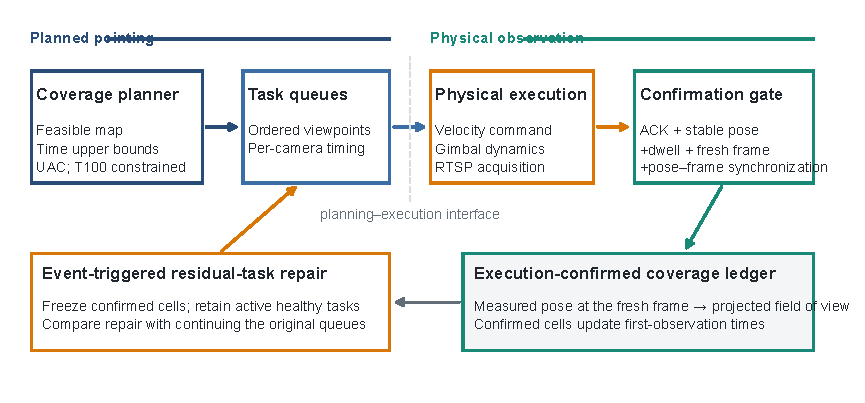
\includegraphics[width=\textwidth]{figure1_system_loop.pdf}
\caption{The ECR-Cover planning--execution--observation loop. Planning produces timed viewpoint queues from a frozen feasible map and end-to-end time bounds. Physical coverage is updated only after command acknowledgment, stable pose, dwell, a fresh usable frame, and pose--frame synchronization. Availability events invoke residual-task repair, but the original queues remain the executable comparison baseline.}\label{fig:system-loop}
\end{figure*}

